\chapter{Architecture and System Design}
		
		\textbf{\textit{dio 1. revizije}}\\

		\textit{ Potrebno je opisati stil arhitekture te identificirati: podsustave, preslikavanje na radnu platformu, spremišta podataka, mrežne protokole, globalni upravljački tok i sklopovsko-programske zahtjeve. Po točkama razraditi i popratiti odgovarajućim skicama:}
	\begin{itemize}
		\item 	\textit{izbor arhitekture temeljem principa oblikovanja pokazanih na predavanjima (objasniti zašto ste baš odabrali takvu arhitekturu)}
		\item 	\textit{organizaciju sustava s najviše razine apstrakcije (npr. klijent-poslužitelj, baza podataka, datotečni sustav, grafičko sučelje)}
		\item 	\textit{organizaciju aplikacije (npr. slojevi frontend i backend, MVC arhitektura) }		
	\end{itemize}

	
		

		

				
		\section{Database}
			
			
		\textit{Database used for this project is a relation based database. Relation is usually referred to as a table that has tuples. Tuple is an object that represents an information. Purpose of the database is easy and fast data manipulation, including saving, deleting, updating and sending data to the server. Database has relations:}
	\begin{itemize}
			\item 	\textit{User)}
			\item 	\textit{Festival)}
			\item 	\textit{Event)}
			\item 	\textit{Specialization)}
			\item 	\textit{WorkerSpec)}
			\item 	\textit{Auction)}
			\item 	\textit{Application)}
			\item 	\textit{Job)}
			\item 	\textit{JobSpec)}
			\item 	\textit{FestivalOrganizers)}



		\end{itemize}
		
			\subsection{Tables details}
			

				\textbf{User} \textit{has entitites for every user of the app. It has all needed personal information about the user and his role.}
				
				\begin{longtabu} to \textwidth {|X[6, l]|X[6, l]|X[20, l]|}
					
					\hline \multicolumn{3}{|c|}{\textbf{User}}	 \\[3pt] \hline
					\endfirsthead
					
					\hline \multicolumn{3}{|c|}{\textbf{User}}	 \\[3pt] \hline
					\endhead
					
					\hline 
					\endlastfoot
					
					\cellcolor{LightGreen}user\_id & INT	&  	User identification number 	\\ \hline
					username	& VARCHAR &  Unique username 	\\ \hline 
					password & VARCHAR & User account password  \\ \hline 
					firstname & VARCHAR	&  Users first name	\\ \hline 
					lastname & VARCHAR	&  Users last name	\\ \hline 
					picture & VARCHAR	&  Profile picture string	\\ \hline 
					phone & VARCHAR	&  Users phone number	\\ \hline 
					email & VARCHAR	&  Users email address	\\ \hline 
					role & VARCHAR	&  Role user will persue in application	\\ \hline
					
				\end{longtabu}

				\textbf{Festival} \textit{contains all needed information about the festival.}
				
				\begin{longtabu} to \textwidth {|X[6, l]|X[6, l]|X[20, l]|}
					
					\hline \multicolumn{3}{|c|}{\textbf{Festival}}	 \\[3pt] \hline
					\endfirsthead

					\hline \multicolumn{3}{|c|}{\textbf{Festival}}	 \\[3pt] \hline
					\endhead
					
					\hline 
					\endlastfoot
					
					\cellcolor{LightGreen}festival\_id & INT	&  	Festival identification number 	\\ \hline
					\cellcolor{LightBlue}creator\_id	& INT &  ID of the user who created the festival 	\\ \hline 
					name & VARCHAR & Festival name  \\ \hline 
					desc & VARCHAR	&  Short festival description, can be empty	\\ \hline 
					logo & VARCHAR	&  Festivals logo string	\\ \hline 
					duration & INTERVAL	&  Festival duration interval	\\ \hline 
					active & BOOLEAN	&  True if festival is active, False if it's unactive	\\ \hline 
					
				\end{longtabu}

				\textbf{Event} \textit{contains information about the event of the festival.}
				
				\begin{longtabu} to \textwidth {|X[6, l]|X[6, l]|X[20, l]|}
					
					\hline \multicolumn{3}{|c|}{\textbf{Event}}	 \\[3pt] \hline
					\endfirsthead
					
					\hline \multicolumn{3}{|c|}{\textbf{Event}}	 \\[3pt] \hline
					\endhead
					
					\hline 
					\endlastfoot
					
					\cellcolor{LightGreen}event\_id & INT	&  	Event identification number 	\\ \hline
					\cellcolor{LightBlue}festival\_id	& INT &  ID of the festival that event belongs to 	\\ \hline 
					\cellcolor{LightBlue}organizer\_id 	& INT &  ID of the user who created the event  	\\ \hline 
					name & VARCHAR & Event name  \\ \hline 
					desc & VARCHAR	&  Short event description, can be empty	\\ \hline 
					location & VARCHAR	&  Events location	\\ \hline 
					start\_Time & TIMESTAMP	&  Event start time	\\ \hline 
					end\_Time & TIMESTAMP	&  Event end time  \\ \hline 
					
				\end{longtabu}


				\textbf{Specialization} \textit{contains all different specializations and their names.}
				
				\begin{longtabu} to \textwidth {|X[7, l]|X[6, l]|X[19, l]|}
					
					\hline \multicolumn{3}{|c|}{\textbf{Specialization}}	 \\[3pt] \hline
					\endfirsthead
					
					\hline \multicolumn{3}{|c|}{\textbf{Specialization}}	 \\[3pt] \hline
					\endhead
					
					\hline 
					\endlastfoot
					
					\cellcolor{LightBlue}specialization\_id & INT	&  	Specializations identification number 	\\ \hline
					name & VARCHAR & Name of the specialization \\ \hline

					
				\end{longtabu}

				\textbf{WorkerSpec} \textit{contains specifications about the user who wants to apply as a worker and his specializations.}
				
				\begin{longtabu} to \textwidth {|X[7, l]|X[6, l]|X[19, l]|}
					
					\hline \multicolumn{3}{|c|}{\textbf{WorkerSpec}}	 \\[3pt] \hline
					\endfirsthead
					
					\hline \multicolumn{3}{|c|}{\textbf{WorkerSpec}}	 \\[3pt] \hline
					\endhead
					
					\hline 
					\endlastfoot
					
					\cellcolor{LightGreen}worker\_id & INT	&  	Workers identification number 	\\ \hline
					\cellcolor{LightBlue}specialization\_id & INT	&  	Specializations identification number 	\\ \hline

					
				\end{longtabu}

				\textbf{Auction} \textit{contains information about auctions.}
				
				\begin{longtabu} to \textwidth {|X[6, l]|X[6, l]|X[20, l]|}
					
					\hline \multicolumn{3}{|c|}{\textbf{Auction}}	 \\[3pt] \hline
					\endfirsthead
					
					\hline \multicolumn{3}{|c|}{\textbf{Auction}}	 \\[3pt] \hline
					\endhead
					
					\hline 
					\endlastfoot
					
					\cellcolor{LightGreen}auction\_id & INT	&  	Auction identification number 	\\ \hline
					start\_Time & TIMESTAMP	&  Auction start time	\\ \hline 
					end\_Time & TIMESTAMP	&  Auction end time  \\ \hline 
					
				\end{longtabu}


				\textbf{Application} \textit{contains information about applications for auctions.}
				
				\begin{longtabu} to \textwidth {|X[8, l]|X[6, l]|X[18, l]|}
					
					\hline \multicolumn{3}{|c|}{\textbf{Application}}	 \\[3pt] \hline
					\endfirsthead
					
					\hline \multicolumn{3}{|c|}{\textbf{Application}}	 \\[3pt] \hline
					\endhead
					
					\hline 
					\endlastfoot
					
					\cellcolor{LightGreen}application\_id & INT	&  	Application identification number 	\\ \hline
					\cellcolor{LightBlue}auction\_id & INT	&  	Auction identification number that worker applies for 	\\ \hline
					\cellcolor{LightBlue}worker\_id & INT	&  	Workers identification number 	\\ \hline
					price & FLOAT & Offered pay for the job \\ \hline
					comment & VARCHAR & Additional comment for application, can be empty \\ \hline
					approximate\_time & INT & Time needed to complete the job, in days \\ \hline
					number\_of\_people & INT & Number of people that will be doing the job \\ \hline

					
				\end{longtabu}
			

				\textbf{Job} \textit{contains information about jobs that had an auction.}
				
				\begin{longtabu} to \textwidth {|X[6, l]|X[6, l]|X[20, l]|}
					
					\hline \multicolumn{3}{|c|}{\textbf{Job}}	 \\[3pt] \hline
					\endfirsthead
					
					\hline \multicolumn{3}{|c|}{\textbf{Job}}	 \\[3pt] \hline
					\endhead
					
					\hline 
					\endlastfoot
					
					\cellcolor{LightGreen}job\_id & INT	&  	Job identification number 	\\ \hline
					\cellcolor{LightBlue}event\_id & INT	&  	Events identification number that job is for\\ \hline
					\cellcolor{LightBlue}worker\_id & INT	&  	Workers identification number that does the job\\ \hline
					\cellcolor{LightBlue}auction\_id & INT	&  	Auctions identification number that auctioned the job\\ \hline
					start\_Time & DATETIME	&  Jobs start time	\\ \hline 
					is\_Completed & BOOLEAN	&  True if job is finished, false if it's still active \\ \hline 

				
				\end{longtabu}


				\textbf{JobSpec} \textit{contains specializations that are needed for the job}
				
				\begin{longtabu} to \textwidth {|X[7, l]|X[6, l]|X[19, l]|}
					
					\hline \multicolumn{3}{|c|}{\textbf{JobSpec}}	 \\[3pt] \hline
					\endfirsthead
					
					\hline \multicolumn{3}{|c|}{\textbf{JobSpec}}	 \\[3pt] \hline
					\endhead
					
					\hline 
					\endlastfoot
					
					\cellcolor{LightGreen}job\_id & INT	&  	Job identification number 	\\ \hline
					\cellcolor{LightBlue}specialization\_id & INT	&  	Specializations identification number 	\\ \hline

					
				\end{longtabu}


				\textbf{FestivalOrganizers} \textit{contains information which user, that is also an organizer, applied for which festival.}
				
				\begin{longtabu} to \textwidth {|X[6, l]|X[6, l]|X[20, l]|}
					
					\hline \multicolumn{3}{|c|}{\textbf{FestivalOrganizers}}	 \\[3pt] \hline
					\endfirsthead
					
					
					\hline 
					\endlastfoot
					
					\cellcolor{LightGreen}festival\_id & INT	&  	Festival identification number 	\\ \hline
					\cellcolor{LightGreen}organizer\_id & INT	&  	Organizers identification number 	\\ \hline
					status & INT	&  \-1 when organizer is waiting on leader, 0 when rejected and 1 when accepted \\ \hline 

				
				\end{longtabu}
			
			\subsection{Database diagrams}
				
				
				\begin{figure}[H]
					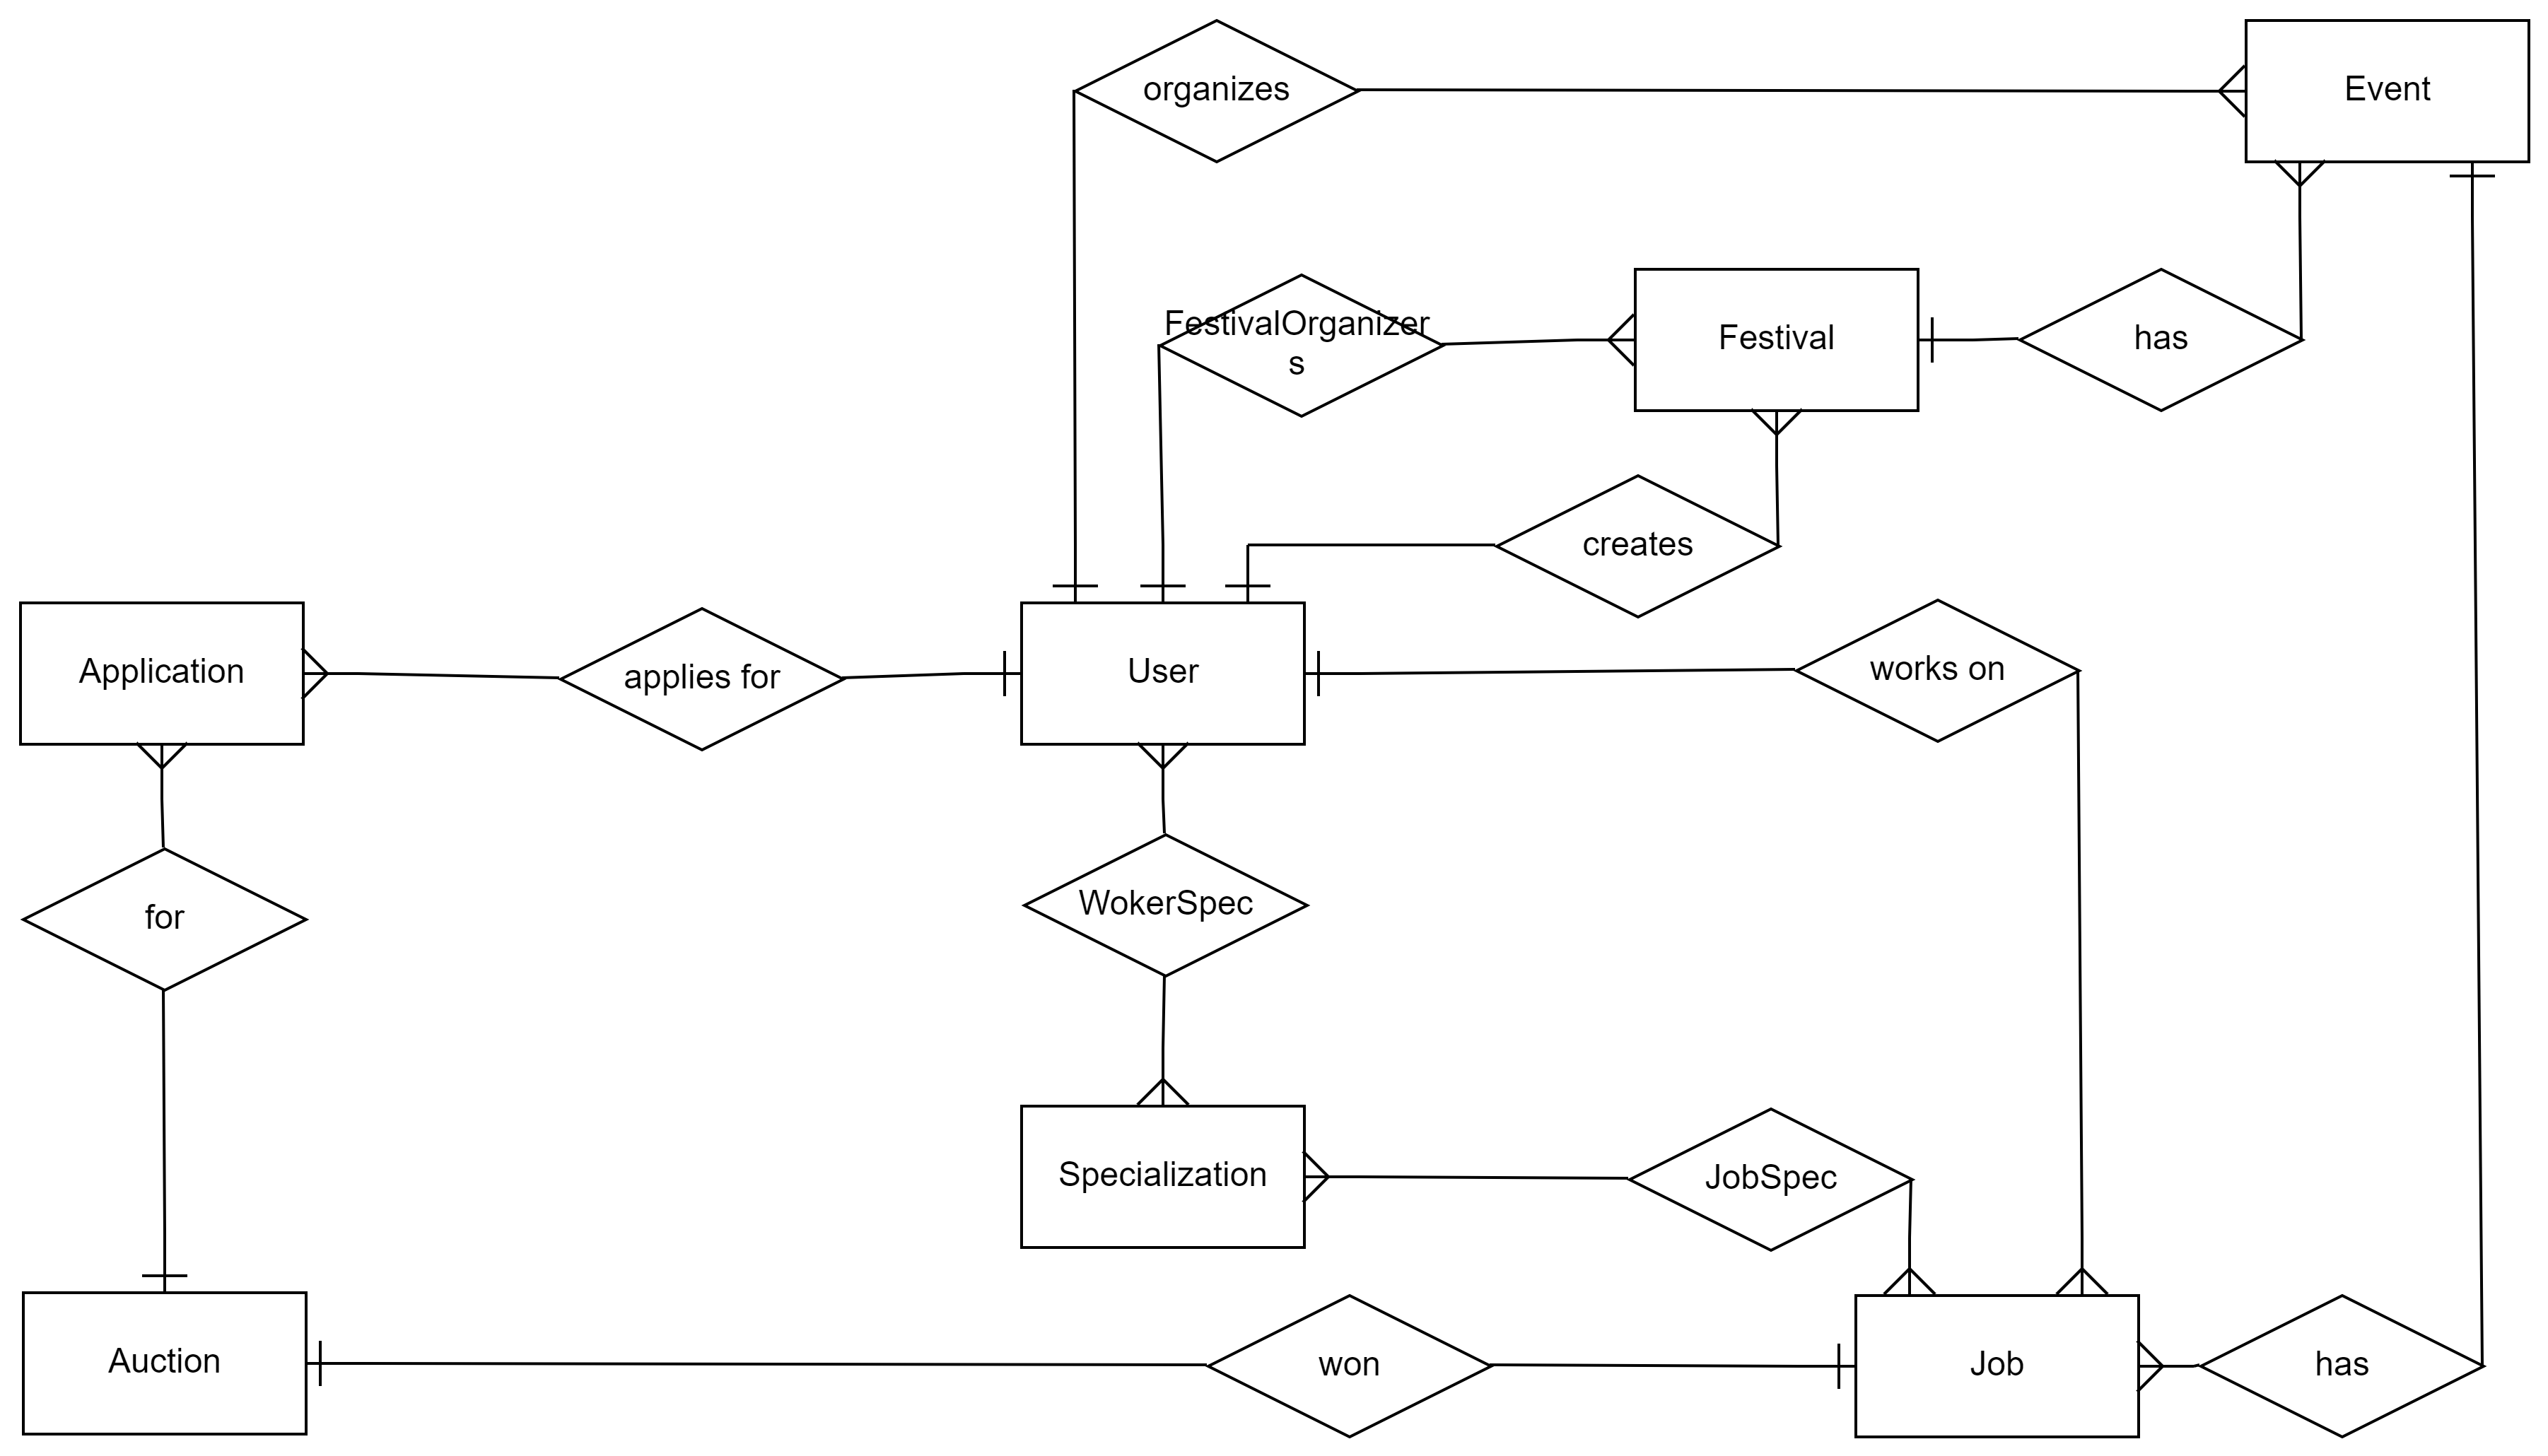
\includegraphics[scale=0.4]{slike/db_er_diag.png}
					\centering
					\caption{E-R Diagram}
					\label{fig:er_diag}
				\end{figure}
			
				\begin{figure}[H]
					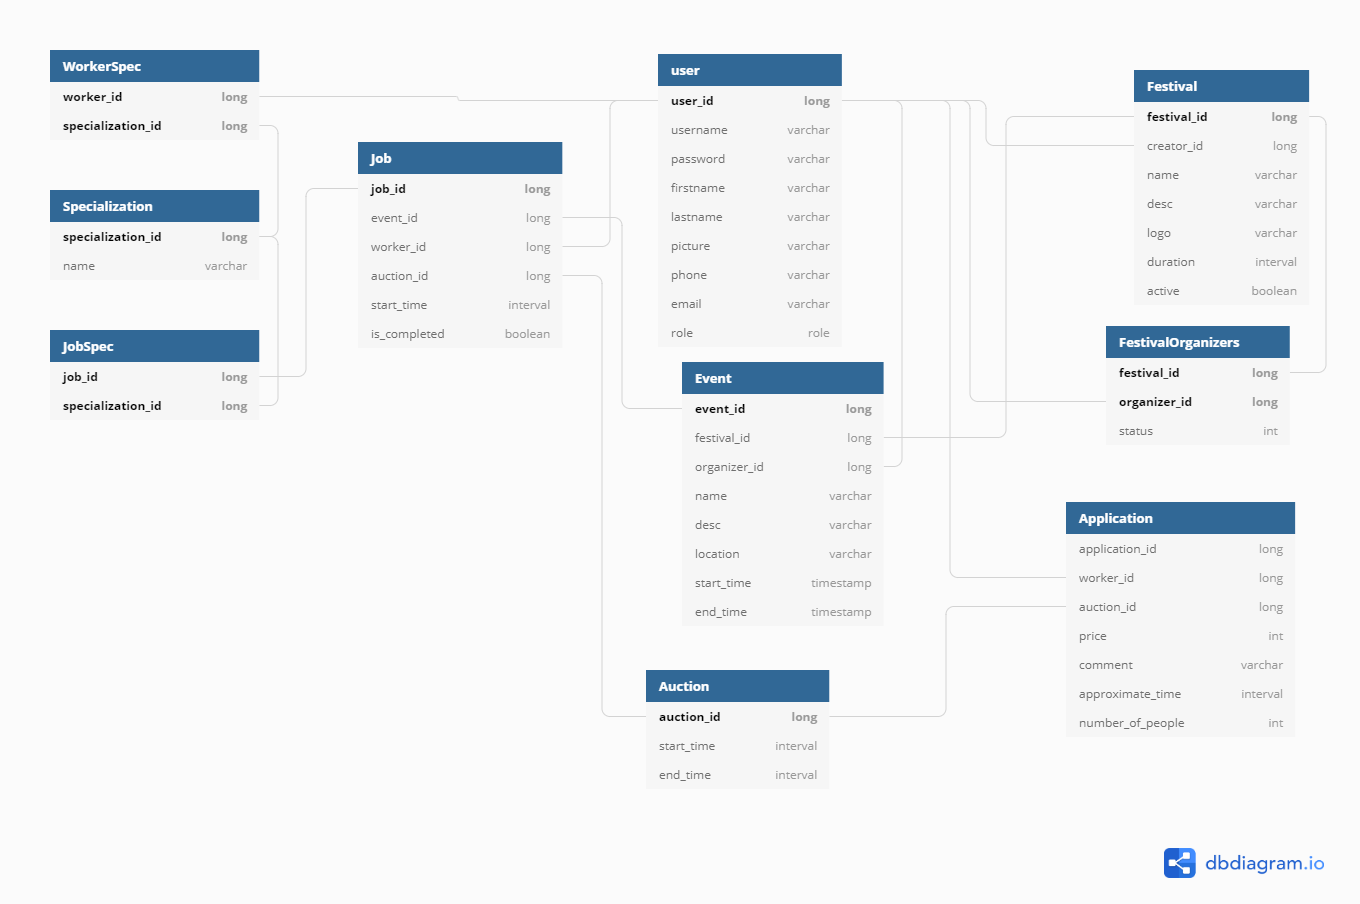
\includegraphics[scale=0.4]{slike/db_normal_diag.png}
					\centering
					\caption{Database Diagram}
					\label{fig:normal_diag}
				\end{figure}
			
			\eject
			
			
		\section{Dijagram razreda}
		
			\textit{Potrebno je priložiti dijagram razreda s pripadajućim opisom. Zbog preglednosti je moguće dijagram razlomiti na više njih, ali moraju biti grupirani prema sličnim razinama apstrakcije i srodnim funkcionalnostima.}\\
			
			\textbf{\textit{dio 1. revizije}}\\
			
			\textit{Prilikom prve predaje projekta, potrebno je priložiti potpuno razrađen dijagram razreda vezan uz \textbf{generičku funkcionalnost} sustava. Ostale funkcionalnosti trebaju biti idejno razrađene u dijagramu sa sljedećim komponentama: nazivi razreda, nazivi metoda i vrste pristupa metodama (npr. javni, zaštićeni), nazivi atributa razreda, veze i odnosi između razreda.}\\
			
			\textbf{\textit{dio 2. revizije}}\\			
			
			\textit{Prilikom druge predaje projekta dijagram razreda i opisi moraju odgovarati stvarnom stanju implementacije}
			
			
			
			\eject
		
		\section{Dijagram stanja}
			
			
			\textbf{\textit{dio 2. revizije}}\\
			
			\textit{Potrebno je priložiti dijagram stanja i opisati ga. Dovoljan je jedan dijagram stanja koji prikazuje \textbf{značajan dio funkcionalnosti} sustava. Na primjer, stanja korisničkog sučelja i tijek korištenja neke ključne funkcionalnosti jesu značajan dio sustava, a registracija i prijava nisu. }
			
			
			\eject 
		
		\section{Dijagram aktivnosti}
			
			\textbf{\textit{dio 2. revizije}}\\
			
			 \textit{Potrebno je priložiti dijagram aktivnosti s pripadajućim opisom. Dijagram aktivnosti treba prikazivati značajan dio sustava.}
			
			\eject
		\section{Dijagram komponenti}
		
			\textbf{\textit{dio 2. revizije}}\\
		
			 \textit{Potrebno je priložiti dijagram komponenti s pripadajućim opisom. Dijagram komponenti treba prikazivati strukturu cijele aplikacije.}